\section{Аналитический обзор литературы}
\subsection{Квантовая динамика двухуровневой системы}
\subsubsection{Формализм оператора плотности}

Согласно постулатам квантовой механики любое квантовое состояние может быть представлено в виде суперпозции (линейной комбинации) состояний называемых собственными:

\begin{equation}
\label{superposition}
|\psi(t)\rangle = \sum_n C_n(t)|\psi_n(t)\rangle,
\end{equation}
\\
\noindent где $C_n$ есть нормированные на единицу амплитуды вероятности обнаружить систему в одном из состояний $|\psi_n(t)\rangle$. Для вычисления математического ожидания некоторой физической величины ей в соответствие ставится линейный эрмитовый оператор:

\begin{eqnarray}
\begin{split}
\label{operator}
\langle A \rangle _t = \langle \psi(t) | A |\psi(t)\rangle = &
  \sum_{n,m} C_m(t) C_n(t) A_{nm} = \\
&= \sum_{n,m} \rho_{n,m}(t) A_{n,m} = Tr (\rho(t), A).
\end{split}
\end{eqnarray} 

Здесь введено дополнительное обозначение: $\rho_{n,m}(t)= C^*_n(t)C_m(t)$  называемое матричным элементом оператора плотности. Смысл его использования становится ясен при рассмотрении систем, для которых нахождение одном из чисто квантовых состояний имеет статистический характер. Введя вероятности $P_i(t)$ нахождения системы в чистых состояниях, можно задать наиболее общее определение матрицы плотности:

\begin{equation}
	\rho = \sum_i P_i(t) |\psi_i\rangle\langle\psi_i|
\end{equation} 

Рассмотрение вычисления математического ожидания для смешанного состояния, когда система изначально может находиться в одном из $|\psi_i(t)\rangle$, даёт следующий результат:

 \begin{equation}
 \begin{split}
 \label{operator}
 \langle A \rangle _t = \sum_i \langle \psi_i(t) | A |\psi_i(t)\rangle = 
 \sum _i \sum_{n,m} P_i(t )C_m(t)& C_n(t) A_{nm} = \\
 &= \sum_{n,m} \rho_{n,m}(t) A_{n,m} = Tr (\rho(t), A).
 \end{split}
 \end{equation} 
 
 Итоговое выражение с точки зрения математики не изменилось, но теперь оно означает проведение сразу двух усреднений. Одно из них учитывает квантово-механическое поведение системы, а другое стохастические процессы, происходящие при взаимодействии с окружением.
 
  Матрица плотности обладает следующими важными свойствами:
 \begin{itemize}
 	\item[a)] $Tr (\rho) = 1$. Это следует из определения;
 	\item[б)] $\rho^2 = \rho$ в случае чистых состояний. Действительно, тогда собственные значения оператора удовлетворяют условию $\rho_i = \rho_i^2$, а значит, из всех возможных квантовых состояний реализует только одно;
 	\item[в)] $Tr(\rho^2) \le 1$. Равенство выполняется в случае чистых состояний. Величину $Tr(\rho^2)$ можно использовать, как характеристику чистоты состояния. 
 \end{itemize} 

  Диагональные элементы матрицы плотности дают информацию о вероятностях обнаружить систему в одном из собственных состояний. Недиагональные элементы никак не влияют на значения математического ожидания наблюдаемых, однако они содержат в себе информацию о когерентности системы. С точки зрения измерения, если они равны нулю, это означает, что не существует такой наблюдаемой, в собственном состоянии которой находится система. Измерения будут давать результаты соответствующие разным собственным состояниям с вероятностями, определяемыми стохастическими процессами связи с окружением.Исключение составляет случай, когда один из диагональных элементов равен единице. 
  
  
  
  \subsubsection{Вектор Блоха и сфера Блоха}
  
  Для любой двухуровневой системы матрица плотности выступает в виде удобной и наиболее общей интерпретации состояния квантовой системы. Так, с её помощью можно дать дополнительное наглядное описание квантового состояния. Любая матрица 2х2 (в том числе и матрица плотности) может быть разложена в линейную комбинацию из единичной матрицы и матриц Паули, имеющих следующий вид:
  
  \begin{equation}
  \sigma_x = \begin{pmatrix} 0 & 1 \\ 1 & 0 \end{pmatrix}; \sigma_y = 
  \begin{pmatrix} 0 & -i \\ i & 0 \end{pmatrix}; \sigma_z = \begin{pmatrix} 1 & 0 \\ 0 & -1 \end{pmatrix};
  \end{equation}
 
  Используя это разложение, можно переписать матрицу плотности следующим образом:
    
\begin{equation}
\label{den_param}
\tag{6}
\rho = \frac{1}{2} \begin{pmatrix}1+R_z & R_x - iR_y \\ R_x + i R_y& 1-R_z\end{pmatrix} = \frac{1}{2}(\mathbb{I}+R_x\sigma_x+R_y\sigma_y+R_z\sigma_z) = \frac{1}{2}\vec R \cdot \vec{\sigma}
\end{equation}

Из условия, что $Tr(\rho^2)\le Tr(\rho)$ следует что:

\begin{equation}
\tag{7}
\begin{split}
Tr (\rho^2) = Tr\frac{1}{4} &
\begin{pmatrix}
(1+R_z)^2+ R_x^2+ R_y^2 & 2(R_x-iR_y) \\ 2(R_x+iR_y)& (1-R_z)^2+R_x^2+R_y^2
\end{pmatrix} = \\
&= \frac{1}{2}(1+R_x^2+R_y^2+R_z^2) \le 1
\end{split}
\end{equation}

Видно, что длина вектора $\vec{R}$ не может быть больше единицы. Поэтому его удобно использовать в наглядной интерпретации состояния системы, а именно, как показано на Рисунке 1, вектора внутри или на поверхности некоторой сферы, называемой сферой Блоха:
\begin{figure}[h]
	\centering
	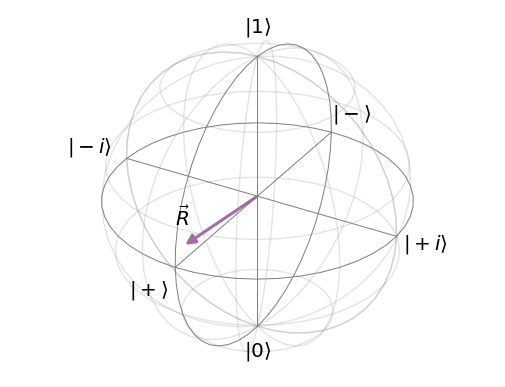
\includegraphics[width=0.4\linewidth]{pictures/Blochvect}
	\caption{Вектор Блоха на сфере Блоха}
	\label{fig:blochvect}
\end{figure}

Далее в работе вектор состояния двухуровневой системы будет обозначаться точками на сфере Блоха.

\subsubsection{Когерентная динамика двухуровневой системы}\label{cohdin}

Унитарная эволюция любой квантовой системы определяется её гамильтонианом, что следует напрямую из уравнения Шрёдингера. Для гамильтониана двухуровневой системы можно повторить приём, использованный в выражении (\ref{den_param}) :

\begin{equation}
\label{Ham}
\tag{8}
\hat H = \frac{\hbar}{2}(\omega_0\hat{\mathbb{I}}+\omega_1\hat\sigma_x+\omega_2\hat\sigma_y+\omega_3\hat\sigma_z) = \frac{\hbar}{2}\vec{\omega}\cdot\vec{\sigma}
\end{equation}
\\

Компонента при $\hat{\mathbb{I}}$ зависит от выбора начала отсчёта энергии и потому может быть опущена. Аналогом уравнения Шрёдингера для матрицы плотности является уравнение Лиувилля-фон-Неймана \cite{Neumann1957}:

\begin{equation}
\tag{9}
\label{liuv}
i\hbar\frac{\partial\hat\rho}{\partial t}=[\hat H, \hat\rho ]
\end{equation}
\\  

Подстановка результатов вычислений (\ref{den_param}) и (\ref{Ham}) в это уравнение приводит к следующему результату:

\begin{equation}
\tag{10}
\dot {\vec R} = \vec \omega \times \vec R
\end{equation}
\\

Это уравнение движения для вектора состояния двухуровневой квантовой системы. Впервые было получено и решено в работе \cite{Feynman1963}. Решением уравнения является чистая прецессия вектора состояния вокруг вектора, соответствующего гамильтониану системы.

В качестве примера будет рассмотрена произвольная двухуровневая система, взаимодействующая с внешней электромагнитной волной. В отсутствии внешнего возбуждения гамильтониан двухуровневой системы:

\begin{equation}
\label{tlsham}
\tag{11}
\hat H = \frac{\hbar\omega_q}{2}(|0\rangle\langle0| - |1\rangle\langle1|) = \frac{\hbar\omega_q}{2}\sigma_z
\end{equation}
\\

Гамильтониан электро-магнитного возбуждения, дипольно связанного с двухуровневой системой есть:

\begin{equation}
\tag{12}
\hat H = \hbar A \cos(\omega_d t) \hat\sigma_x , 
\end{equation}

\noindent а итоговый гамильтониан системы имеет следующий матричный вид:

\begin{equation}
\tag{13}
\hat H = \frac{\hbar}{2}\begin{pmatrix} \omega_q & A(e^{i\omega_d t} + e^{-i\omega_d t})\\ A(e^{i\omega_d t} + e^{-i\omega_d t})& -\omega_q \end{pmatrix}
\end{equation}
\\

Для того чтобы сделать задачу стационарной необходимо перейти в систему координат, вращающуюся с частотой внешней волны, делается это следующим унитарным преобразованием:

\begin{equation}
\label{unittr}
\tag{14}
\hat U = e^{\frac{i}{\hbar}\omega_d t\sigma_z}  = \begin{pmatrix}
e^{\frac{i}{2}\omega_d t} & 0 \\0& e^{-\frac{i}{2}\omega_d t}
\end{pmatrix}
\end{equation}
\\

Новый Гамильтониан вычисляется по формуле, напрямую следующей из уравнения Шрёдингера:

\begin{equation}
\tag{15}
\label{rabres}
\tilde{\hat H} = \hat U \hat H \hat U^\dagger+i\dot{\hat U}\hat U^\dagger 
\end{equation}




\noindent и имеет вид (более подробное решение описано в \cite{Gu2017}):

\begin{equation}
\tag{16}
\tilde{\hat{H}} = \frac{\hbar}{2}
\begin{pmatrix}
	\omega_q - \omega_d & A\\
	A&			\omega_d - \omega_q 
\end{pmatrix}
\end{equation}
\\
Для получения этого результата было использовано так называемое приближение вращающейся волны. Плоско-поляризованная внешняя волна, представляется как суперпозиция двух волн с круговой поляризацией. Преобразование (\ref{unittr}) переводит в систему отсчёта, связанную с одной из двух волн. Считается, что вторая волна, имея в новой системе отсчёта нерезонансную частоту не вносит серьёзного вклада. Из выражения (\ref{rabres}) видно, что состояние системы под действием внешней волны будет вращаться вокруг направления вдоль оси $X$ на сфере Блоха, как показано на Рисунке 2.
\begin{figure}[!h]
	\centering
	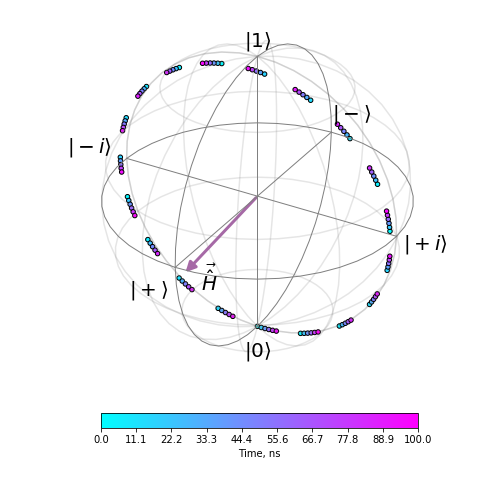
\includegraphics[width=0.4\linewidth]{pictures/Rabi}
	\caption{Динамика квантового состояния под воздействием внешнего излучения}
	\label{fig:rabi}
\end{figure}

Это периодическое изменение состояния называется осцилляциями Раби. Во-первых видно, что ввиду наличия некоторой отстройки частоты сигнала от частоты перехода в системе $(\omega_q - \omega_d \ne 0)$ система не может быть переведена в состояние $|1\rangle$ с вероятностью 100 \%. Во-вторых такая картина даёт информацию о необходимых длительностях сигналов переводящих систему в различные квантовые состояния. 

\subsubsection{Некогерентная динамика. Открытые системы}\label{neun}
Как уже было сказано, матрица плотности даёт возможность учитывать не только чисто квантовые особенности поведения системы, но и неунитарные процессы, происходящие из-за взаимодействия с классическим окружением \cite{Budini2009,Talkner2009}. Любая система в той или иной степени является открытой, т.е. взаимодействует с окружением. Гамильтониан в наиболее общем случае имеет вид:
\begin{equation}
\tag{17}
\hat H_{SE} = \hat H_S + \hat H_E + \hat H_I 
\end{equation} 	
Здесь $\hat H_S$ - гамильтониан системы, $\hat H_E$ - гамильтониан окружения и, наконец, $\hat H_I$ - гамильтониан их взаимодействия. Эволюция системы всё ещё определяется выражением (\ref{liuv}), но и гамильтониан матрица плотности в нём теперь отражают состояние системы вместе с окружением. Т.е. уравнение принимает вид:
\begin{equation}
\tag{18}
\label{rhose}
i\hbar\frac{\partial\hat\rho_{SE}}{\partial t}= [\hat H_{SE},\hat\rho_{SE}]
\end{equation}
\\

Для того чтобы представить уравнение (\ref{rhose}) в виде выражения, описывающего унитарную эволюцию системы с дополнительным слагаемыми отвечающим за неунитарную эволюцию необходимо сделать ряд последовательных приближений:
\begin{itemize}
	\item [a)] воздействие окружения на систему считается слабым возмущением. А само окружение представляется в виде набора бозонных мод, так что его гамильтониан имеет вид: $\hat H = \sum_n \hbar\omega_n \hat a^\dagger_n\hat a$;
	\item [б)] состояние окружения считается постоянным и равновесным. В этом случае эволюция системы и эволюция окружения - статистически-независимые процессы и матрицу плотности $\hat \rho_{SE}$ можно представить в виде $\hat \rho_{SE} = \hat \rho_{S}\otimes\hat\rho_E$;
	\item[в)] характерные времена изменения матрицы плотности системы считается существенно меньше  корреляционных времён, связанных с процессами внутри системы, так что эволюция матрицы плотности определяется только её текущим состоянием и никак не зависит от предшествующих; 
\end{itemize}	

Применение приближений для изменения вида уравнения ({\ref{liuv}}) - громоздкая процедура, она подробно описана в работе \cite{Vool2017}. В результате в нём появляются слагаемые, отвечающие за отличие эволюции системы от унитарной. Итоговое уравнение имеет форму Линдблада:
\begin{equation}
\tag{19}
\label{lindblad}
i\hbar \frac{\partial\hat\rho}{\partial t} = [\hat H,\rho] + \sum_n (2\hat L_a \hat \rho \hat L^\dagger_n - \{\hat L^\dagger_n\hat L_n,\hat \rho\})
\end{equation} 
\\

Здесь $\hat L_n$ и $\hat L^\dagger_n$ - операторы Линдблада, вид которых подбирается в каждой конкретной задаче. В них содержится информация о механизмах и скоростях рассматриваемых процессов. В качестве примера будет рассмотрено несколько вариантов неунитарной эволюции двухуровневой системы. 

Для первого примера вид оператора Линдблада имеет вид:
\begin{equation}
\tag{20}
\label{dephaseop}
\hat L = \hat L^\dagger = \sqrt{\gamma}\hat \sigma^\dagger\hat \sigma^-  = \sqrt{\gamma}\begin{pmatrix}
1&0\\0&0\
\end{pmatrix}
\\
\end{equation}

После подстановки уравнение (\ref{lindblad}) представляет собой матричное дифференциальное уравнение:
\begin{equation}
\tag{21}
\begin{pmatrix}
\dot\rho_{00} & \dot\rho_{01}\\\dot\rho_{10}&\dot\rho_{11}
\end{pmatrix} = \begin{pmatrix}
0&-\gamma\rho_{01}\\-\gamma\rho_{10}&0
\end{pmatrix}
\end{equation}

Его решение даёт следующий результат:
\begin{equation}
\tag{22}
\hat\rho(t) = \begin{pmatrix}
\rho_{00}(0)&\rho_{01}(0)e^{-\gamma t}\\ \rho_{10}(0)e^{-\gamma t}&\rho_{11}(0)
\end{pmatrix}
\end{equation}

Такой вид неунитарной эволюции называется чистой дефазировкой. В этом случае диагональные элементы остаются постоянными, а недиагональные экспоненциально убывают во времени, скорость затухания при это определяется параметром $\gamma$. Чистота состояния так же убывает экспоненциально:

\begin{equation}
\tag{23}
tr\hat\rho^2(t) = \rho_{00}^2(0) +\rho_{11}^2(0) + |\rho_{01}^2(0)|e^{-2\gamma t}
\end{equation} 

Динамика состояния в этом случае будет иметь вид изображённый на Рисунке 3:
	
\begin{figure}[h]
	\centering
	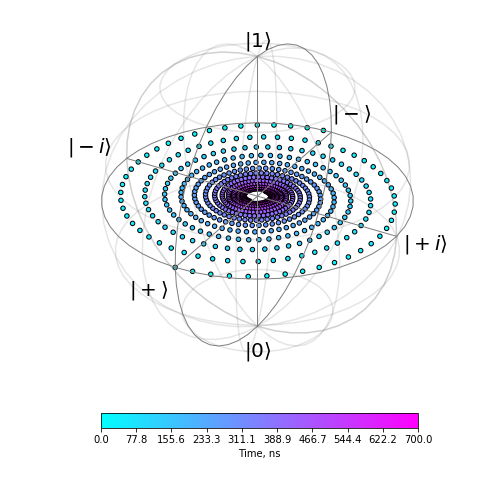
\includegraphics[width=0.4\linewidth]{pictures/Puredephase}
	\caption{Чистая дефазировка квантового состояния $|+\rangle$ на сфере Блоха}
	\label{fig:puredephase}
\end{figure}

В качестве второго примера будет рассмотрено влияние операторов Линдблада вида:
\begin{equation}
\label{relaxop}
\tag{24}
\begin{split}
&\hat L = \sqrt{\Gamma/2}\hat\sigma^\dagger- = \sqrt{\Gamma/2}
\begin{pmatrix}
0&1\\0&0
\end{pmatrix}\\
&\hat L^\dagger = \sqrt{\Gamma/2}\hat\sigma_- = \sqrt{\Gamma/2}
\begin{pmatrix}
0&0\\1&0
\end{pmatrix}
\end{split}
\end{equation}

Подстановка в (\ref{lindblad}) даёт матричное уравнение:
\begin{equation}
\tag{25}
\begin{pmatrix}
\dot\rho_{00}&\dot\rho_{01}\\
\dot\rho_{10}&\dot\rho_{11}
\end{pmatrix} =
\begin{pmatrix}
\Gamma\rho_{00}&-(\Gamma/2) \rho_{01}\\
-(\Gamma/2)\rho_{10} & -\Gamma\rho_{11}
\end{pmatrix},
\end{equation}

\noindent решение которого имеет вид:
\begin{equation}
\label{relax}
\tag{25}
\hat\rho(t) = 
\begin{pmatrix}
1-\rho_{11}(0)e^{-\Gamma t}& \rho_{01}(0)e^{(-\Gamma/2)t}\\
\rho_{10}(0)e^{(-\Gamma/2)t}&\rho_{11}(0)e^{-\Gamma t}
\end{pmatrix}
\end{equation}

С течением времени недиагональные элементы матрицы экспоненциально стремятся к нулю. На диагонали $\rho_{11}$, а $\rho_{00}$ - к единице. В дополнение к дефазировке, выражение (\ref{relax}) описывает так называемый процесс релаксации, т.е. передачи энергии из системы в связанное с ней окружение.
Интересно заметить, что эволюция берёт свой старт в чистом состоянии $|-\rangle$ и под действием неунитарных процессов, постепенно проходя через смешанное состояние, снова стремится к чистому состоянию $|0\rangle$. 

 Динамика квантового состояния $|-\rangle$ под действием оператора (\ref{relaxop}) представлена на Рисунке 4:

\begin{figure}[h]
	\centering
	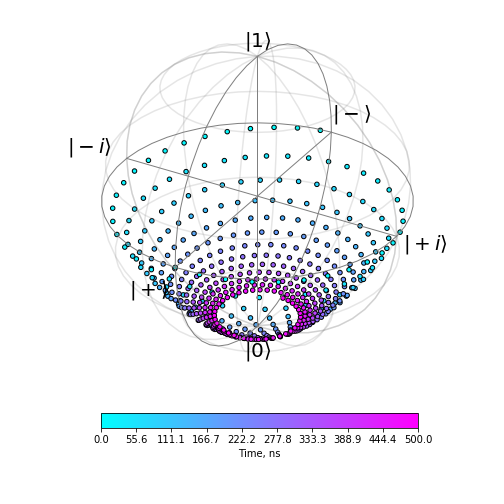
\includegraphics[width=0.4\linewidth]{pictures/Relaxation}
	\caption{Релаксация квантового состояния $|-\rangle$ на сфере Блоха}
	\label{fig:relaxation}
\end{figure}

Наконец, если учесть воздействие сразу двух операторов Линдблада (\ref{relaxop}) и (\ref{dephaseop}), решение уравнения (\ref{lindblad}) будет иметь вид:

\begin{equation}
\tag{26}
\hat \rho(t)= 
\begin{pmatrix}
\rho^e_{00}+(\rho_{00}(0)-\rho^e_{00})e^{-\Gamma t}&\rho_{01}(0)e^{-(\Gamma/2+\gamma)t}\\\rho_{10}(0)e^{-(\Gamma/2+\gamma)t} &
\rho^e_{11}+(\rho_{11}(0)-\rho^e_{11})e^{-\Gamma t}
\end{pmatrix}
\end{equation} 

Здесь $\rho^e_{00}$ и $\rho^e_{11}$ - некоторые равновесные заселённости квантовых состояний. Их значения могут быть расчитаны для каждой температуры T из соотношения: $\frac{\rho^e_{11}}{\rho^e_{00}}=e^{-\frac{\hbar\omega_q}{k_BT}}$.

Динамика квантового состояния в этом случае изображена на Рисунке 5: 
\begin{figure}[!h]
	\centering
	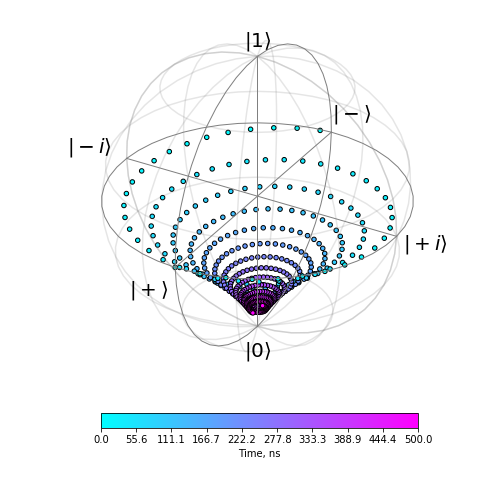
\includegraphics[width=0.4\linewidth]{pictures/Relaxdephase}
	\caption{Процессы релаксации и дефазировки квантового состояния $|-\rangle$ на сфере Блоха}
	\label{fig:relaxdephase}
\end{figure}

\subsection{Трансмон}\label{transmon}

На данный момент существует целый спектр физических реализаций двухуровневых систем \cite{Gershenfeld1997,Jaksch2000,Buluta2011}. Одним из наиболее развиваемых сильнейшими в мире лабораториями является направление, основанное на сверхпроводящих устройствах \cite{Yan2016,Martinis2009,DeGraaf2018}. Об одном из таких устройств и пойдёт речь в этой главе. 

Первично идея зарядового кубита была предложена в работе \cite{Nakamura1999}. Схема реализации представлена на Рисунке 6:
\begin{figure}[h]
	\centering
	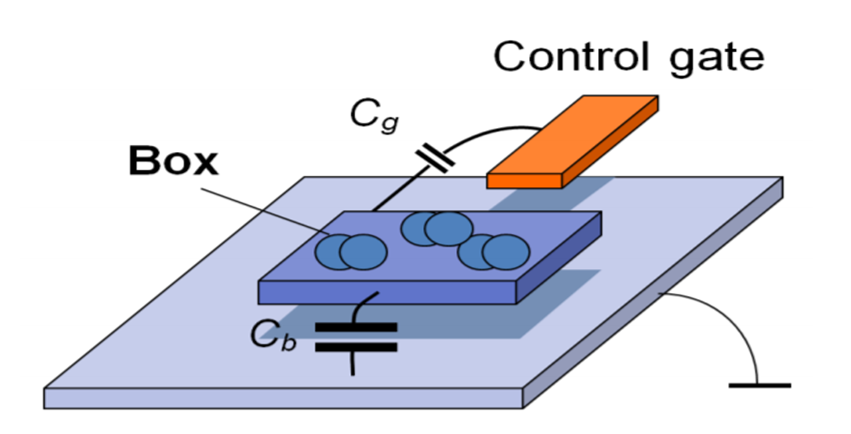
\includegraphics[width=0.6\linewidth]{pictures/chargequbit}
	\caption{Зарядовый кубит \cite{Shulga2017}}
	\label{fig:chargequbit}
\end{figure}

К небольшому сверхпроводящему островку (Box), ёмкостно связанному со сверхпроводящией плоскостью (землёй), подводится контролирующее напряжение (Control gate). При достижении низких температур число куперовских на островке квантуется.  С помощью изменения напряжения на Control gate можно получить ситуацию, когда состояния с разным числом куперовских пар на острове вырождаются. Вырождение снимается, если куперовские пары получают возможность тунелировать на землю за счёт эффекта Джозефсона \cite{Wendin2005}. Величина расщепления в первом приближении равна энергии, необходимой куперовской паре на тунелирование. Итоговый гамильтониан системы состоит из зарядового и Джозефсоновского вклада и может быть записан в виде:

\begin{equation}
\hat H = E_C (\hat n - n_g)^2 - E_J \cos {\hat \phi}, 
\label{cpb1}
\tag{27}
\\
\end{equation}

\noindent где $E_C = \frac{(2e)^2}{2C_q}$ - зарядовая энергия, а $E_J = \frac{\Phi_0 I_C}{2\pi}$ - Джозефсоновская энергия. Так же в выражении  (\ref{cpb1}) присутствуют операторы числа куперовских пар на островке - $\hat n_g$  и фазы волновой функции сверхпроводящего состояния $\hat \phi$. При низких температурах для них выполняется коммутационное соотношение: 

\begin{equation}
\label{commut}
\tag{28}
[\hat n, \hat \phi ] = i
\end{equation}

Используя (\ref{commut}) можно переписать гамильтониан (\ref{cpb1}) в виде:

\begin{equation}
\tag{29}
\label{cpb}
\hat H  = \sum_n [E_C(n-n_g)^2]|n\rangle\langle n| - \frac{E_j}{2}(|n\rangle\langle n+1|+|n+1\rangle\langle n|)]
\end{equation} 


На Рисунке 7 приведён результат численной диагонализации гамильтониана (\ref{cpb}) для разных соотношений $E_j/ E_c$. Полученные состояния являются функциями напряжения на Control gate (или заряда $n_g$).
\begin{figure}[h]
	\centering
	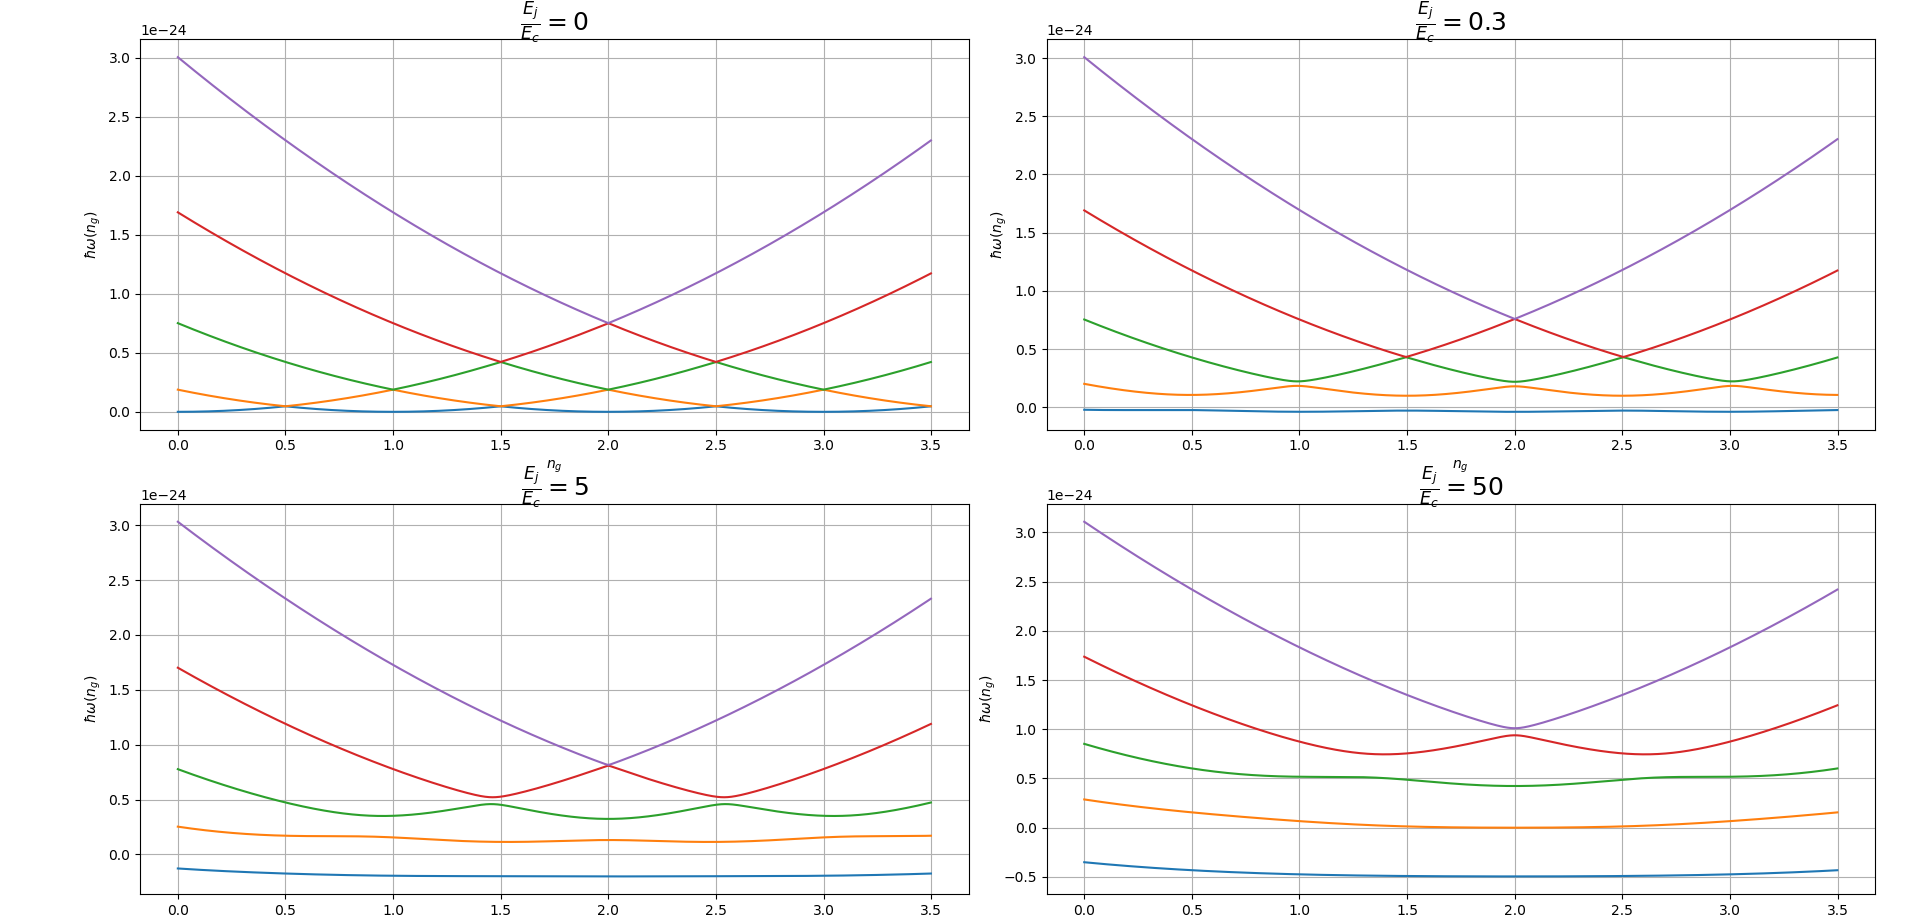
\includegraphics[width=0.9\linewidth]{pictures/cpb}
	\caption{Спектральные линии зарядового кубита}
	\label{fig:cpb}
\end{figure}

Видно, что в случае отсутствия Джозефсоновской энергии спектральные линии пересекаются. При её появлении вырождение снимается, но до тех пор пока преобладает зарядовая энергия наблюдается сильная зависимость энергии состояний от наведённого заряда, что, как было показано в (\ref{neun}) ведёт к дополнительной дефазировке.  Проблема была решена в работе \cite{Koch2007}. Был создан кубит-трансмон. С помощью большой шунтирующей ёмкости удалось  получить соотношение $\frac{E_J}{E_C}  \sim 50$ и избавиться таким образом от зарядовой дисперсии. Как видно из Рисунка 7, энергетическая структура в этом случае представляет собой неэквидистантные уровни ангармонического осциллятора. Из теории возмущения можно рассчитать поправки к частотам переходов:

\begin{equation}
\tag{30}
\begin{split}
&E_{01}= \sqrt{8E_JE_C}- E_C\\
&E_{12}= \sqrt{8E_JE_C}-2E_C
\end{split}
\end{equation}  

Частоту перехода в кубите так же можно контролировать, используя СКВИД \cite{Kleiner2004}. При манипуляции близкими по частоте перехода импульсами систему можно приближённо считать двухуровневой, а гамильтониан (\ref{cpb}) привести к виду:

\begin{equation}
\label{spinham}
\tag{31}
\hat H = -\frac{E_c}{2}(1-2 n_g)\hat \sigma_z - \frac{E_j}{2}\hat\sigma_x, 
\\
\end{equation}

\noindent который является полностью аналогичным виду гамильтониана самой распространённой двухуровневой системы, а именно одиночного спина $\frac{1}{2}$ в постоянном внешнем магнитном поле. 

\subsection{Трансмон связанный с резонатором} \label{transres}
Реализация любых вычислительных алгоритмов подразумевает возможность считать итоговый результат\cite{Wallraff2005}. Не являются исключением и алгоритмы квантовой информатики, которые базируются на возможности двухуровневой системы находиться в когерентной суперпозиции собственных состояний. 

Идея считывания квантовых состояний одиночных кубитов пришла из науки, которая называется квантовая электродинамика в полости (Cavity QED \cite{Blais2004}). Рассматривается система, изображённая на Рисунке 8:
\begin{figure}[h]
	\centering
	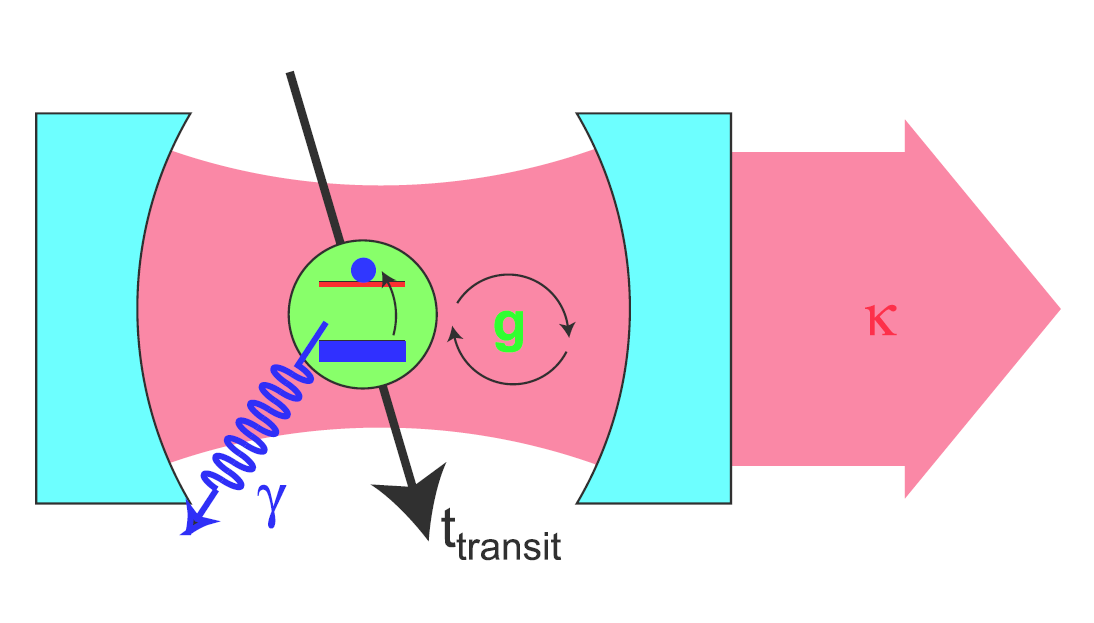
\includegraphics[width=0.5\linewidth]{pictures/qed}
	\caption{Система QED}
	\label{fig:qed}
\end{figure}

Она состоит из двух зеркал с распространяющимися между ними модами электромагнитного поля. Через зеркала пропускают пучок атомов. Эволюция системы определяется рядом параметров: $\gamma$ - декремент затухания заселённости возбуждённого состояния атома, определяется величиной связи атома с модами полей, в которые можно отдать энергию, $k$ - обратное время спонтанного излучения фотона из полости, определяется связью системы с континуумом мод за пределами полости, $g$ - сила связи моды полости с атомом, определяется величиной дипольного взаимодействия между ними. 

Естественно, что для создания универсального вычислительного устройства на основе механизмов квантовой механики необходима куда более масштабируемая система с идентичной энергетической структурой. Один из вариантов такой структуры рассмотрен в задаче квантовой электродинамике цепей (Circuit QED) и  изображён на  Рисунке 9.

Так же для наглядности на Рисунке 10 приведена оптическая фотография чипа, с физически реализованной системой.

Вместо системы зеркал здесь представлен участок передающей линии с разрывами на концах. Являясь по сути последовательностью LC- контуров, эта система представляет собой резонатор, частота которого определяется геометрическими параметрами. В область повышенной амплитуды поля помещён кубит Трансмон дипольно связанный с модой поля.


\begin{figure}[!h]
	\centering
	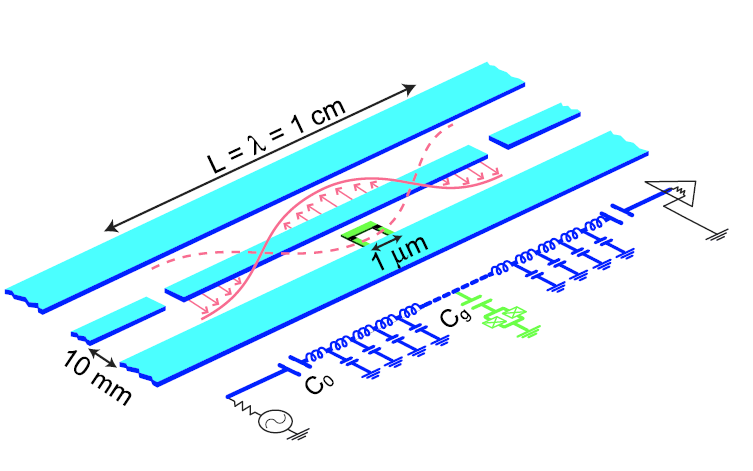
\includegraphics[width=0.5\linewidth]{pictures/qed1}
	\caption{Схема Circuit QED}
	\label{fig:qed1}
\end{figure}


\begin{figure}[h]
	\centering
	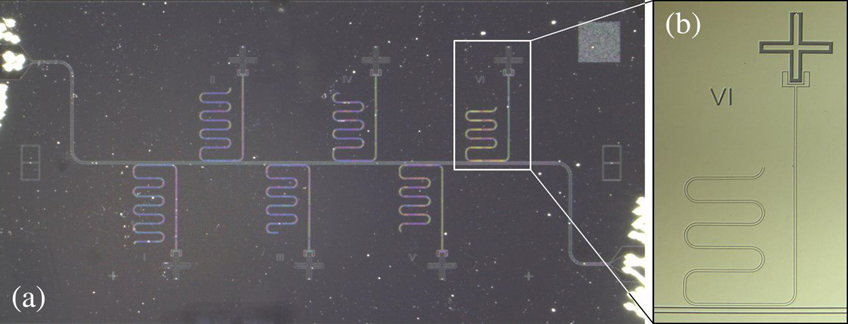
\includegraphics[width=0.5\linewidth]{pictures/chip}
	\caption{Чип с системой резонаторов и кубитов}
	\label{fig:chip}
\end{figure}

Эквивалентная электронная схема системы изображена на Рисунке 11:
\begin{figure}[!h]
	\centering
	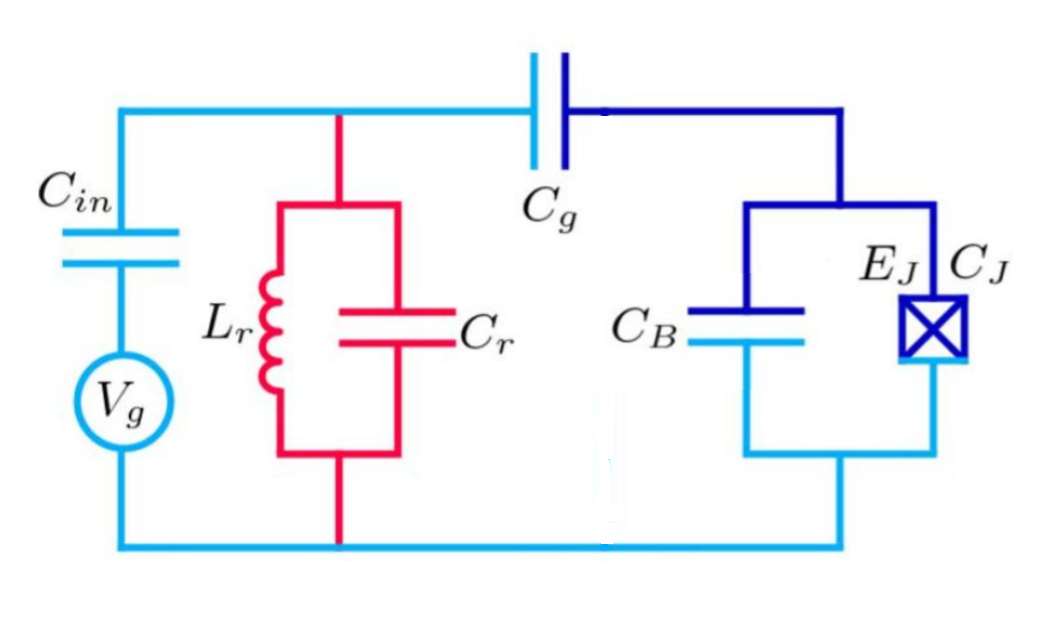
\includegraphics[width=0.5\linewidth]{pictures/electr}
	\caption{Эквивалентная электрическая схема кубита и резонатора}
	\label{fig:electr}
\end{figure}

Эволюция такой системы, а так же необходимость использования резонаторов для считывания квантовых состояний становится ясной при рассмотрении модели Джейнса-Каммингса \cite{Clarke2008}, согласно которой гамильтониан такой системы может быть представлен в виде:
\begin{equation}
\label{JCham}
\tag{32}
\hat H = \hbar\omega_r(\hat a ^\dagger \hat a +\frac{1}{2})-\frac{\hbar\omega_a}{2}\hat \sigma_z + \hbar g(\hat a^\dagger\hat\sigma^-+ \hat a\hat\sigma^\dagger) + \hat H_\gamma + \hat H_K
\\
\end{equation}

Здесь первое слагаемое - гамильтониан гармонического осциллятора, отвечающего резонаторной моде поля, второе - гамильтониан двухуровневой системы, третье - гамильтониан их взаимодействия. С физической точки зрения слагаемые $\hat a^\dagger\hat\sigma^-$  и $\hat a \hat\sigma^\dagger$ отвечают переходу возбуждения из кубита в резонатор и наоборот. $\hat H_k $ и $\hat H_\gamma$, как было указано ранее, отвечают за спонтанное излучение возбуждения из резонатора и атома соотвественно. Ввиду наличия связи состояния, отвечающие возбуждению в кубите или резонаторе, не являются собственными для оператора (\ref{JCham}). Происходит гибридизация и новые собственные состояния определяются, как линейная комбинация исходных $(\alpha|0,n\rangle+\beta|1,n-1\rangle)$.
Комплексные числа $\alpha$  и $\beta$ могут быть найдены из решения уравнения на собственные значения и собственные векторы указанного гамильтониана:
\begin{equation}
\tag{33}
\begin{split} 
\hat H &(\alpha|0,n\rangle+\beta|1,n-1\rangle) = E (\alpha|0,n\rangle+\beta|1,n-1\rangle) \iff\\
&\alpha\hbar\omega_r(n+\frac{1}{2})|0,n\rangle+\beta\hbar\omega_r(n-\frac{1}{2})|1,n-1\rangle - a\frac{\hbar\omega_q}{2}|0,n\rangle+\beta\frac{\hbar\omega_q}{2}|1,n-1\rangle + \\&\hbar g\sqrt{n}(\beta|0,n\rangle+\alpha|1,n-1\rangle)= E(\alpha|0,n\rangle+\beta|1,n-1\rangle)
\\
\end{split}
\end{equation}

Приравнивая коэффициенты при одинаковых состояния, можно получить:
\begin{equation}
\tag{34}
\begin{split}
&\alpha (\omega_r n +\frac{\Delta}{2}-\frac{E}{\hbar})+g\sqrt n \beta = 0\\
&\alpha g\sqrt n + (\omega_r n - \frac{\Delta}{2} - \frac{E}{\hbar})\beta  = 0 
\end{split}
\end{equation}

Здесь $\Delta = \omega_r - \omega_q$. Из определителя этой системы можно найти собственные значения гамильтониана:

\begin{equation}
\tag{35}
\frac{E}{\hbar}=\omega_r n \pm \sqrt{\frac{\Delta^2}{4}-g^2 n}
\\
\end{equation}

Как указывалось ранее практический интерес представляет режим работы системы, при котором $\Delta >>g$. В этом случае $n<<(\frac{\Delta}{2g})^2$ тогда второе слагаемое можно разложить в ряд Тейлора по параметру $(\frac{\Delta}{2g})^2$:

\begin{equation}
\tag{36}
\label{eighval}
\frac{E}{\hbar} = \omega_r n \pm \frac{\Delta}{2}(1- n \frac{g^2}{2\Delta^2})
\\
\end{equation}
В этом приближении выражения для собственных состояний системы имеют вид:
\begin{equation}
\tag{37}
\begin{split}
&|-,0\rangle = -\frac{g}{\Delta}|1,0\rangle + |0,1\rangle\\
&|+,1\rangle = |1,0\rangle + \frac{g}{\Delta}|0,1\rangle
\end{split}
\end{equation}
Наконец, подставив (\ref{eighval}) выражение для оператора числа возбуждений в системе:
\begin{equation}
\tag{38}
\hat n = -\frac{1}{2}(\hat \sigma_z +1)+\hat a^\dagger\hat a,
\end{equation}
\noindent можно получить:
\begin{equation}
\label{JChamD}
\tag{39}
\hat H_d = \hbar(\omega_r + \frac{g^2}{\Delta}\hat\sigma_z)\hat a ^\dagger\hat a + \frac{\hbar}{2}(\omega_q +\frac{g^2}{\Delta})\hat\sigma_z
\\
\end{equation}

Итоговый гамильтониан в дисперсионном режиме содержит две важные особенности. Во-первых, резонансная частота резонатора зависит от состояния кубита. Этот эффект называет дисперсионным сдвигом \cite{Stammeier}. Во-вторых, частота перехода в кубите, зависит от числа фотонов в резонаторе (эффект Штарка \cite{Kox2013}). Энергетическая структура системы при наличии отстройки изображена на Рисунке 12:

\begin{figure}[h]
	\centering
	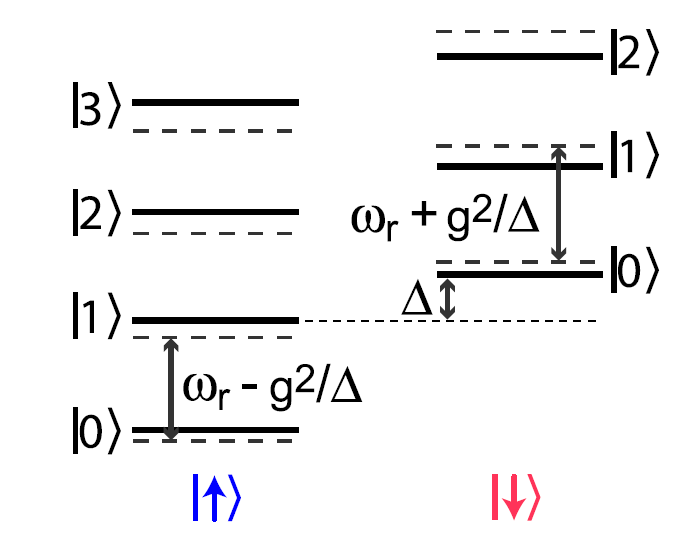
\includegraphics[width=0.5\linewidth]{pictures/JCenergy}
	\caption{Энергетическая структура системы cQED в дисперсионном режиме}
	\label{fig:jcenergy}
\end{figure}

Таким образом, частота резонансного отклика системы кубит+резонатор на внешнее возбуждение зависит от состояния кубита, как показано на Рисунке 13.
\begin{figure}[!h]
	\centering
	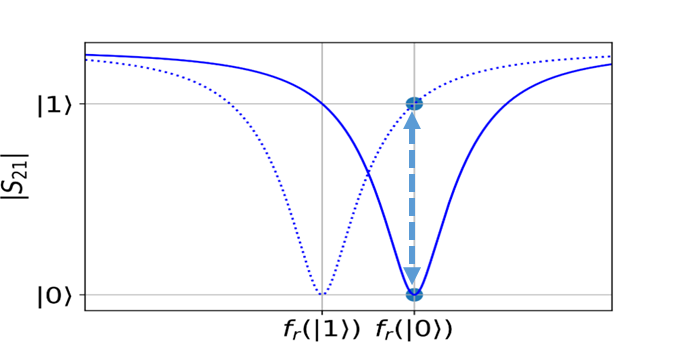
\includegraphics[width=0.5\linewidth]{pictures/dispshift}
	\caption{Дисперсионный сдвиг}
	\label{fig:dispshift}
\end{figure}
 
Зависимость частоты резонатора от состояния кубита лежит в основе дисперсионного считывания \cite{Chen2012} и двухтоновой спектроскопии \cite{Leng2011}. 

\subsection{Дисперсионное считывание. Квадратурные модуляция и демодуляция}
Для считывания квантовых состояний двухуровневых систем необходимо уметь генерировать короткие импульсы на частоте резонатора. Для этого  в работе использовались квадратурные смесители (IQ-Mixers). Это устройства, работающие по схеме, изображённой на Рисунке 14.

\begin{figure}[h]
	\centering
	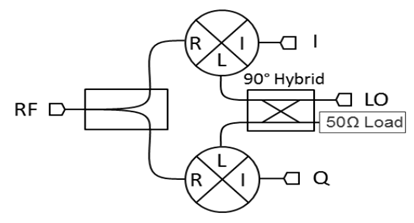
\includegraphics[width=0.5\linewidth]{pictures/IQ-mixer}
	\caption{Схема работы квадратурного смесителя}
	\label{fig:iq-mixer}
\end{figure}
На канал RF подётся гармонический сигнал. На каналы I и Q можно подавать сигналы любой необходимой формы. Сигнал на выходе LO, задаётся соотношением:
\begin{equation}
\tag{40}
U_{LO}(t) = I(t)\sin{\omega t}+ Q_(t)\cos{\omega t}
\end{equation}

Во-первых, подавая на каналы I и Q сигналы прямоугольной формы, можно получить короткие импульсы на обеих квадратурах, контролирующие состояние кубита, подобно тому, как это было описано в (\ref{cohdin}). 

Во-вторых, на канал LO можно принимать сигнал на выходе из образца, и с помощью каналов I и Q можно разделять его на составляющие соответствующие обеим квадратурам. Эти процессы называются модуляцией и демодуляцией сигнала соответственно.

Дисперсионное считывание представляет собой отправку одинаковых сигналов через образец на канал LO и напрямую из генератора на канал RF и его последующую демодуляцию. Результат такой демодуляции представлен на Рисунке 15:

\begin{figure}[!h]
	\centering
	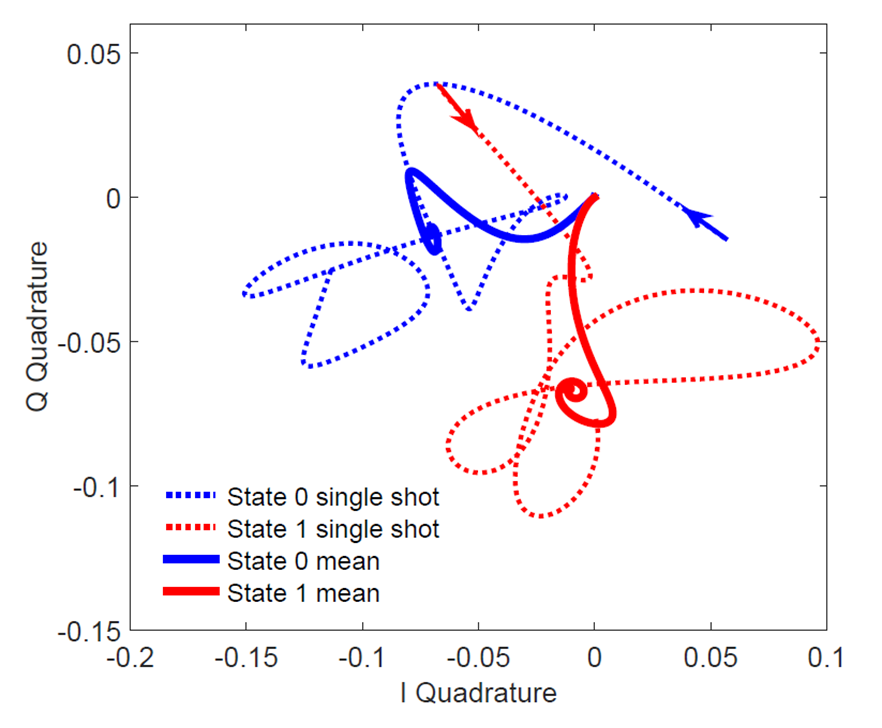
\includegraphics[width=0.5\linewidth]{pictures/readout}
	\caption{Временная развёртка сигнала в IQ-пространстве \cite{Magesan2015} }
	\label{fig:readout}
\end{figure}

По существу это измерение величины напряжение на каналах I и Q миксера в каждый момент времени. Очевидно, что вид таких "траекторий"  зависит резонансной частоты резонатора, а значит и от состояния кубита. 
   